% This is samplepaper.tex, a sample chapter demonstrating the
% LLNCS macro package for Springer Computer Science proceedings;
% Version 2.20 of 2017/10/04
%
\documentclass[runningheads]{llncs}
%
\usepackage{graphicx}
% Used for displaying a sample figure. If possible, figure files should
% be included in EPS format.
%
% If you use the Hyperref package, please uncomment the following line
% to display URLs in blue roman font according to Springer's eBook style:
% \renewcommand\UrlFont{\color{blue}\rmfamily}

\usepackage{orcidlink} % Orcid links
% Fix underscore in dois
\usepackage[strings]{underscore}

% Listing settings
\usepackage{listings}
\usepackage{xcolor}

\lstdefinelanguage{Interaction}[]{Java}{
    comment=[l]{---},
}

\lstset{emph={
    synchronize
    },emphstyle={\color{blue}\bfseries}
}

\begin{document}
% https://www.discotec.org/2024/coordination
% Regular papers 7-15 pages + references
% Artifacts using Zenodo together with this repo. Maybe a big CSV file with our classification results is input for some plots (clustering). Then, the source code for that should also be added.
\title{Classifying coordination approaches}
%
%\titlerunning{Abbreviated paper title}
% If the paper title is too long for the running head, you can set
% an abbreviated paper title here
%
\author{Tim Kr\"{a}uter\inst{1}\orcidlink{0000-0003-1795-0611} \and
Julien Deantoni\inst{2}\orcidlink{0000-0001-6962-7846}
Adrian Rutle\inst{1}\orcidlink{0000-0002-4158-1644} \and
Harald K\"{o}nig\inst{3,1}\orcidlink{0000-0001-6304-6311} \and
Yngve Lamo\inst{1}\orcidlink{0000-0001-9196-1779}}
%
\authorrunning{T. Kräuter et al.}
% First names are abbreviated in the running head.
% If there are more than two authors, 'et al.' is used.
\institute{Western Norway University of Applied Sciences, Bergen, Norway  \\
\email{tkra@hvl.no, aru@hvl.no, yla@hvl.no} \and
University Cote d’Azur, Sophia Antipolis, France \\
\email{julien.deantoni@univ-cotedazur.fr} \and
University of Applied Sciences, FHDW, Hanover, Germany\\
\email{harald.koenig@fhdw.de}}
%
\maketitle              % typeset the header of the contribution
%
\begin{abstract}
TODO
\keywords{
ADL \and
Coordination language \and
Coordination framework \and
Co-Simulation \and
Feature model
}
\end{abstract}

\section{Introduction} \label{sec:introduction}

% Categorizing ADLs, Coordination languages, Co-simulation, and Coordination frameworks (BCOOL and me).

% Paper outline

% What was our search methodology? Google Scholar? Other databases? Which search terms/queries?
% ADL/Architecture description language & survey/classification/literature review

\section{Categories of Coordination Approaches} \label{sec:approaches}

\autoref{fig:overview} gives an overview of the different categories of coordination approaches.
% TODO: Describe the overview layer/level by level.

\begin{figure}[ht]
	\centering
	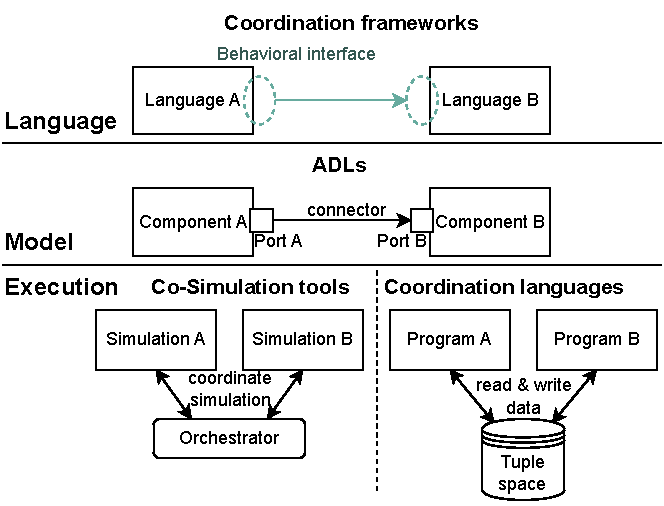
\includegraphics[width=0.7\textwidth]{images/overview}
	\caption{Overview of coordination approaches}
	\label{fig:overview}
\end{figure}

In the following sections, we will describe each of the categories: ADLs, coordination languages, Co-Simulation tools, and coordination frameworks in detail.

\subsection{Architecture Description Languages}
% General idea
Architecture Description Languages (ADLs) aim to describe the structure of systems, allowing developers to focus on high-level components and their connections rather than lines of source code~\cite{clementsSurveyArchitectureDescription1996,medvidovicClassificationComparisonFramework2000,medvidovicFrameworkClassifyingComparing1997}.
% What is an ADL and what is not?
Many different ADLs have been proposed in the academic literature and by the industry~\cite{medvidovicClassificationComparisonFramework2000,woodsArchitectureDescriptionLanguages2005}.
Nevertheless, clearly defining what an ADL is becomes challenging due to overlap with general-purpose modeling languages~\cite{clementsSurveyArchitectureDescription1996}.

% Describing ADLs generally.
The three buildings blocks of ADLs are defined as: (1) \textit{components}, (2) \textit{connectors}, (3) \textit{architectural configuration}~\cite{medvidovicClassificationComparisonFramework2000,medvidovicFrameworkClassifyingComparing1997}.
% Component
A \textit{component} is a unit of computation or data repository~\cite{medvidovicClassificationComparisonFramework2000}.
Components vary in size, ranging from representing individual services to entire systems.

% Connector
\textit{Connectors} serve as architectural elements to model interactions between components and the regulations that oversee those interactions~\cite{medvidovicClassificationComparisonFramework2000}.
A difference to components is that connectors must not be implemented as distinct entities such as message brokers but can also represent shared variables or links between applications realized by client-server protocols \cite{medvidovicClassificationComparisonFramework2000}.

% Architectural configuration
\textit{Architectural configuration}, also known as topology, represents the structural arrangement of components and connectors in a connected graph, defining the overall architecture~\cite{medvidovicClassificationComparisonFramework2000}.
This structure determines if the combined semantics results in the desired behavior.
For example, one can check for deadlocks and starvation.

% ADLS are formal and usually incorporate one formal language. Usually, a process algebra. They do not support multiple formal specification languages cite medvidovicClassificationComparisonFramework2000.
In addition, ADLs usually incorporate a formal semantics/language to enable analysis.


% The formal semantics is a distinguishing factor to say UML/ArchiMate are considered as modeling languages not as ADLs in this paper.
For this paper, we consider only ADLs which incorporate a formal semantics and thus do not consider other modeling languages such as UML \cite{objectmanagementgroupUnifiedModelingLanguage2017} and ArchiMate \cite{theopengroupArchiMateSpecification2023} which can be seen as ADLs.




% Give examples that we use later Wright/Darwin and MontiArc
% Cite ADLs.

% "No ADL provides explicit support for multiple formal specification languages."
\cite{medvidovicClassificationComparisonFramework2000}

% Commonaltities listed are nice: formally-defined semantics, lack of real-world applications <.<
\cite{clementsSurveyArchitectureDescription1996}

% "ADLs are still not mainstream, i.e., used by practitioners."
% Good description of ADLs such as Darwin and Wright with citations and examples.
% "ADLs usually use process algebras, which practitioners do not like."
\cite{ozkayaAreWeThere2013}


% ADLs vanished, but UML didn't, which people did not accept as an ADL!
% In academia, an ADL has to allow for some formal analysis or something, which UML doesn't. We stick to the academic definition and do not consider UML or Archimate to be ADLs in this paper. But yeah, both languages are used heavily to describe software architectures.
\cite{pandeyArchitecturalDescriptionLanguages2010}

\subsection{Coordination Languages}
% Define Coordination language and give examples
% Cite and survey

\subsection{Co-Simulation Tools}
% Define Co-Simulation and give examples
\cite{gomesCoSimulationSurvey2019}

\subsection{Coordination Frameworks}
% Define Coordination-framework and give examples
% Cite and survey?
\cite{varalarsenBCOolBehavioralCoordination2016,varalarsenBehavioralCoordinationOperator2015}~\cite{krauterBehavioralConsistencyMultimodeling2023}

% Maybe add the overview from Julien and me here to help with the definition

\section{Feature model} \label{sec:features}
% Cut up the feature model and describe it in dedicated subsections (maybe the first layer of nodes after the root)
% Maybe add a full feature model as an artifact (use GitHub repo with Zenodo)

\begin{figure}[ht]
	\centering
	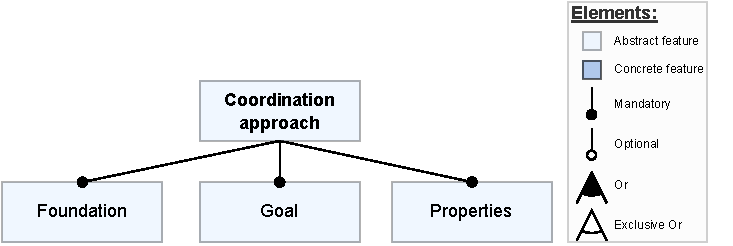
\includegraphics[width=1\textwidth]{images/root}
	\caption{Feature Model Overview}
	\label{fig:feature_model_root}
\end{figure}

\subsection{Coordination}
\subsection{Goal}
\subsection{Properties}

\section{Classification examples} \label{sec:classifications}

% Classify some representatives, sticking to the same order as in the preliminaries.
\subsection{MontiArc} % ADL representative
\subsection{Lingua Franca} % Coordination language representative
\subsection{Co-Simulation example} % Co-Simulation representative
\subsection{BCOOL} % Coordination framework representative
\subsection{BCorrLang} % Coordination framework representative --> Need to classify my approach for the thesis

\section{Classification results}
% Clusters of features for ADL, Coordination language, Co-Simulation, and coordination frameworks?
% Maybe they can somehow be visualized nicely using some clusters with overlaps (vann diagram or something)

% Commonalities between clusters

% Differences between clusters

% What are the unique features of each approach? Does this match their intended usage scenarios?

\section{Running example}
% I'm not sure about this section yet, but a running example would be nice to show in different approaches.

\lstinputlisting[
label=lst:interactions,
language=Interaction,
caption=Interactions for the running example]{listings/interactions.txt}

\section{Conclusion} \label{sec:conclusion}

\bibliographystyle{splncs04}
\bibliography{bib}

\end{document}
